\clearpage
\section{Entropy Estimator}

\begin{refsection}

\begin{tcolorbox}	
\begin{tabular}{p{2.75cm} p{0.2cm} p{10.5cm}} 	
\textbf{Students Name} &:& Gustavo Anjos \\
\textbf{Goal}          &:& Simulate binary entropy estimator.\\
\textbf{Directory}     &:& sdf/eit\_42256\_estimator\_entropy
\end{tabular}
\end{tcolorbox}

The concept of entropy was formulated by the first time in 1948 by Claude Shannon in the article entitled
"A Mathematical Theory of Communication". In this work Shannon defined entropy as the average amount of
information generated by a random source, stating that the events that occur less should carry more information
than the ones the occur often.
In the following sections the theoretical description of the implemented entropy estimator (binary) is provided
and evaluated using a simple simulation chain. 

\subsection{Theoretical Analysis}

Defining \textit{p} as the probability of the outcome '1', the binary entropy \textit{h} is formulated as 

\begin{equation}
h = -p\log_2(p) - (1-p)\log_2(1-p)
\end{equation}

The amount of information associated to the event '1' is quantified by $\log_2({\frac{1}{p}})$, while in the case of the
outcome '0', this amount of information is given by $\log_2({\frac{1}{1-p}})$. As formulated above, the entropy generated 
by a binary source is obtained making the expectation of the amount of information generated by the events '0' and '1'.
      
\begin{figure}[h]
\subsection*{}
    \centerline{
       \includegraphics[scale=0.50]{figures/bin_entropy_th.png}
    }
    \caption{Binary Entropy}
\end{figure}

As depicted in the figure above, the binary entropy is a symmetric concave function with the maximum reached when the
probability of the outcomes '0' and '1' is equal to 0.5, i.e. when the source is uniform.  
	 
	 
\subsection{Simulation Analysis}

In order to evaluate the developed estimator, a simple simulation chain formed by a binary generator and a sink block
was implemented as shown in the following figure. The input of the estimator block is feeded with a binary stream
generated by an independent random source configured to generate '0' with a predefined probability.  

\begin{figure}[h]
\subsection*{}
    \centerline{
       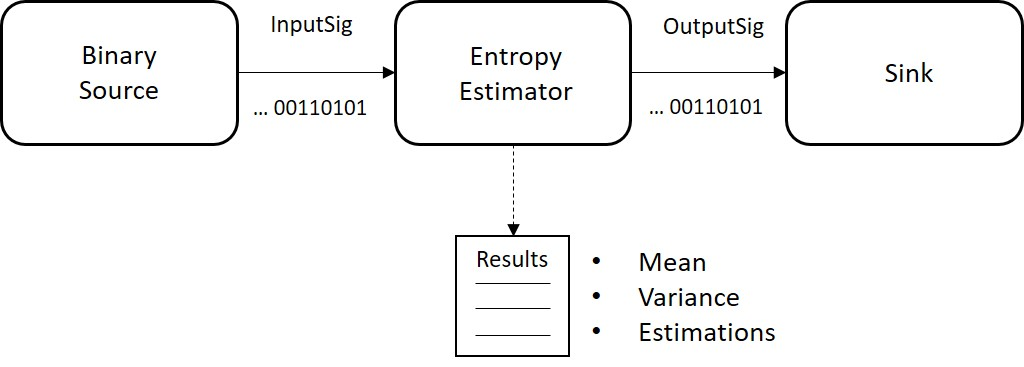
\includegraphics[scale=0.55]{figures/system_block_diagram.jpg}
    }
\end{figure}

After configuring the minimum window size (minWindow) and the total n? of bits to be considered by the estimator block 
(nBits), the mean and the variance of the entropy estimations regarding the input signal are writen to a file. During the
estimation process the input is transferred to the output buffer without changes.  

The simulation parameters applied at the binary source as well in the entropy estimator are defined bellow. The buffer size at the input of the estimator block was set to 
300 bits, being all the other parameters configured to the default value.

\begin{table}[H]
\centering
\label{tb:paramsource}
\begin{tabular}{|c|c|c|}
\hline
\textbf{Parameter}                      & \textbf{Default Value}                                       \\ \hline
mode                          			& Random                                                       \\ \hline
probabilityOfZero                		& 0:0.1:1                                                      \\ \hline
numberOfBits                          	& 100000                                                       \\ \hline

\end{tabular}
\caption{Binary Source Parameters}
\end{table}


\begin{table}[H]
\centering
\label{tb:paramestimator}
\begin{tabular}{|c|c|c|}
\hline
\textbf{Parameter}                      & \textbf{Default Value}                                        \\ \hline
nBits                          			& 90000                                                         \\ \hline
minWindow                				& 1000                                                      	\\ \hline

\end{tabular}
\caption{Entropy Estimator Parameters}
\end{table}

\textbf{Parameters Description}: The parameter 'minWindow' allows the user to set the 
minimum window size for each individual estimation. If 'minWindow' is lower than the 
input buffer size, the estimator adjusts the window to the size of the input buffer, 
otherwise the window is rounded to a multiple of the input buffer size, ensuring always 
that the window is greater or equal than 'minWindow'. The total number of bits processed 
by the estimator is equal to the largest value that is a multiple of the window size and 
is not greater than the input parameter 'nBits'.

\paragraph{}
The following table defines the system signals used in the implementation of the simulation chain.
\begin{table}[H]
\centering
\label{tb:signals}
\begin{tabular}{|c|c|c|}
\hline
\textbf{Signal name}                            & \textbf{Signal type}                      \\ \hline
S0                                              &  Binary    								\\ \hline
S1                                              &  Binary    								\\ \hline
\end{tabular}
\caption{System Signals}
\end{table}

The header and the source files required to the implementation of the described chain are
defined in the following tables.

\begin{table}[H]
\centering
\label{tb:signalsh}
\begin{tabular}{|c|c|c|}
\hline
\textbf{File name}                              & \textbf{Description}                                                          & \textbf{Status} \\ \hline
netxpto\_20180118.h                             &                                                                               &    \checkmark   \\ \hline
binary\_source\_20180523.h       				&Binary random generator                                                       	&    \checkmark   \\ \hline
entropy\_estimator\_20180715.h                  &Entropy estimator                                                 				&    \checkmark   \\ \hline
sink\_20180118.h                                &Sink                                                                           &    \checkmark   \\ \hline
\end{tabular}
\caption{Header Files}
\end{table}

\begin{table}[H]
\centering
\begin{tabular}{|c|c|c|}
\hline
\textbf{File name}                              & \textbf{Description} 		& \textbf{Status} \\ \hline
netxpto\_20180118.cpp                           &                      		&    \checkmark   \\ \hline
binary\_source\_20180523.cpp     				&Binary random generator    &    \checkmark   \\ \hline
entropy\_estimator\_20180715.h                  &Entropy estimator          &    \checkmark   \\ \hline
sink\_20180118.cpp      						&Sink                      	&   \checkmark   \\ \hline

\end{tabular}
\caption{Source Files}
\label{tb:signalss}
\end{table}


\subsection{Simulation Results}
For a buffer size of 300 bits at the input of the estimator block, and taking into account the parameters 
defined above, the estimator adjusts the window size to 1200 bits 
and analyzes a total of 90000 bits.

In the following table and figure, the theoretical entropy \textit{h} is compared with the entropy values
computed by the implemented estimator.

\paragraph{}

\begin{table}[H]

\centering
\begin{tabular}{| l | l | l | l | l | l | l | l | l | l | l | l |}
    \hline
    1-\textit{p} & 0 & 0.1 & 0.2 & 0.3 & 0.4 & 0.5 & 0.6 & 0.7 & 0.8 & 0.9 & 1 \\ \hline
    \textit{h} & 0 & 0.469 & 0.721  & 0.881  & 0.971 & 1 & 0.971 & 0.881 & 0.721 & 0.469 & 0 \\ \hline 
	M & 0 & 0.463 & 0.723 & 0.879 & 0.969 & 0.999 & 0.969 & 0.880 & 0.717 & 0.464 & 0 \\ \hline    
    V & 0 & 81 & 58 & 23 & 8.1 & 0.08 & 6.7 & 20 & 49 & 71 & 0 \\ \hline
\end{tabular}
\caption{Theoretical entropy \textit{h}, entropy mean (M) and variance (V$*10^{-5}$) at the estimator output}
\end{table}


\begin{figure}[H]
\subsection*{}
    \centerline{
       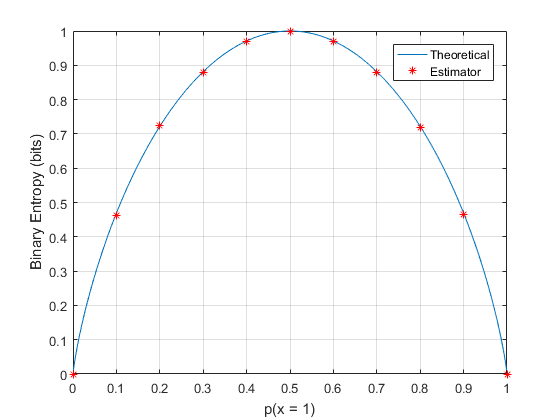
\includegraphics[scale=0.60]{figures/Bin_entropy_results.png}
    }
\caption{Binary Entropy Results (mean)}
\end{figure}

As can be seen, the numerical results computed by the entropy estimator matched the expected theoretical values.  

\paragraph{}

\subsection*{Open Issues}

\newpage


% bibliographic references for the section ----------------------------
\clearpage
\printbibliography[heading=subbibliography]
\end{refsection}
\addcontentsline{toc}{subsection}{Bibliography}
\cleardoublepage
% --------------------------------------------------------------------- 